\section{Theoretical Results}


\begin{table}
\centering
\caption{Properties of simulated clusters.}
\begin{tabular}{lrrrccc}
\toprule
name                 & Xe atoms & Ar atoms & Xe \% &   ICD                &  ETMD                & $\Gamma_{ICD,ETMD}$\\
\midrule
ArXe\_2\_1atom       &      1   &     12   &  7.7  &      0.0             &  0.0                 &     0.0            \\
ArXe\_3\_1atom       &      1   &     54   &  1.8  &      0.0             &  0.0                 &     0.0            \\ 
ArXe\_3\_2atom       &      2   &     53   &  3.6  & 3.346$\cdot 10^{-6}$ & 1.666$\cdot 10^{-5}$ & 2.006$\cdot 10^{-5}$ \\
ArXe\_8\_1layer      &   1415   &    642   & 68.8  & 7.039$\cdot 10^{-4}$ & 2.573$\cdot 10^{-4}$ & 9.612$\cdot 10^{-4}$ \\
\midrule
XeAr\_2\_surface     &      1   &     13   &  7.1  & 7.922$\cdot 10^{-5}$ & 0.0                  & 7.922$\cdot 10^{-5}$ \\
XeAr\_2\_edge        &      1   &     13   &  7.1  & 1.320$\cdot 10^{-6}$ & 0.0                  & 1.320$\cdot 10^{-6}$ \\
XeAr\_2\_vertex      &      1   &     13   &  7.1  & 5.013$\cdot 10^{-6}$ & 0.0                  & 5.013$\cdot 10^{-6}$ \\
XeAr\_2\_2top        &      2   &     13   & 13.3  & 1.011$\cdot 10^{-5}$ & 1.513$\cdot 10^{-5}$ & 2.523$\cdot 10^{-5}$ \\
XeAr\_2\_2midtop     &      2   &     13   & 13.3  & 1.588$\cdot 10^{-5}$ & 7.686$\cdot 10^{-7}$ & 1.665$\cdot 10^{-5}$ \\
XeAr\_2\_2endtop     &      2   &     13   & 13.3  & 1.587$\cdot 10^{-5}$ & 1.772$\cdot 10^{-7}$ & 1.605$\cdot 10^{-5}$ \\
XeAr\_3\_surface     &      1   &     55   &  1.8  & 6.371$\cdot 10^{-6}$ & 0.0                  & 6.371$\cdot 10^{-6}$ \\
XeAr\_3\_edge        &      1   &     55   &  1.8  & 4.791$\cdot 10^{-6}$ & 0.0                  & 4.791$\cdot 10^{-6}$ \\
XeAr\_3\_vertex      &      1   &     55   &  1.8  & 2.701$\cdot 10^{-6}$ & 0.0                  & 2.701$\cdot 10^{-6}$ \\
XeAr\_3\_edge\_in    &      1   &     54   &  1.8  & 7.708$\cdot 10^{-6}$ & 0.0                  & 7.708$\cdot 10^{-6}$ \\
XeAr\_3\_vertex\_in  &      1   &     54   &  1.8  & 5.258$\cdot 10^{-6}$ & 0.0                  & 5.258$\cdot 10^{-6}$ \\
XeAr\_3\_2in         &      2   &     53   &  3.6  & 1.166$\cdot 10^{-5}$ & 5.453$\cdot 10^{-6}$ & 1.711$\cdot 10^{-5}$ \\
XeAr\_3\_6in         &      6   &     49   & 10.9  & 3.746$\cdot 10^{-5}$ & 4.050$\cdot 10^{-5}$ & 7.796$\cdot 10^{-5}$ \\
XeAr\_3\_6\_scat     &      6   &     49   & 10.9  & 2.923$\cdot 10^{-5}$ & 6.737$\cdot 10^{-5}$ & 9.660$\cdot 10^{-5}$ \\
\bottomrule
\end{tabular}
\label{table:theo_gammas}
\end{table}

\begin{figure}[h]
 \centering
 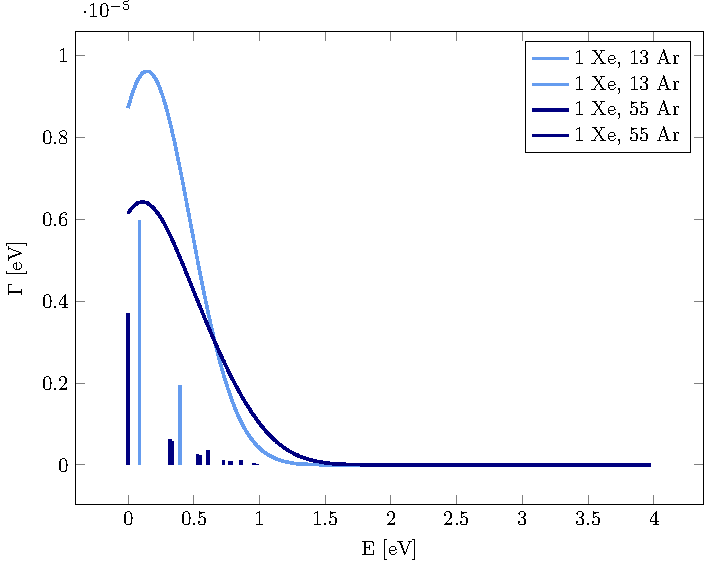
\includegraphics[width=8.5cm]{pics/surf.pdf}\\
 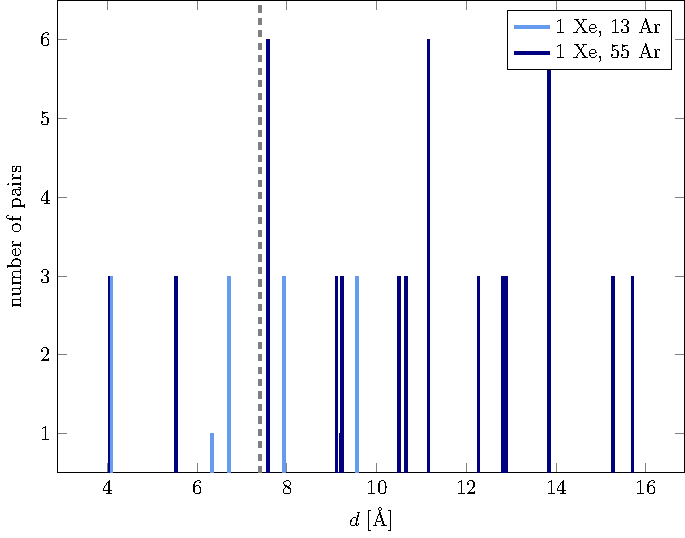
\includegraphics[width=8.5cm]{pics/R_comp.pdf}
 \caption{Panel 1: Simulated electron-electron coincidence spectra
          for argon clusters
          consisting of 13 and 55 atoms with on additional xenon atom residing
          on top of one of the argon surfaces.\\
          Panel 2: Distribution of Ar-Xe distances $d$ in the studied ArXe
          clusters. The ICD channels open at \unit[7.58]{\AA} and
          \unit[36.00]{\AA}, respectively. Hence only pairs at longer interatomic
          distances than the gray line contribute to the coincidence spectra.
          The distance distribution of the larger cluster contains larger
          distances which correspond to peaks at higher kinetic energies of
          the ICD electron in the coincidence spectra (Panel 1).}
 \label{figure:surf}
\end{figure}


\begin{figure}[h]
 \centering
 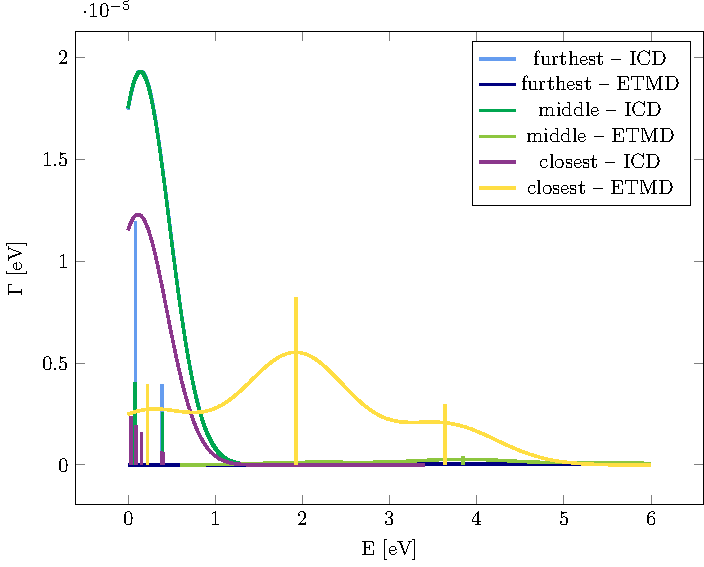
\includegraphics[width=8.5cm]{pics/2tops.pdf}
 \caption{Simulated coincidence spectra of argon clusters consisting of 13
          argon atoms with 2 additional xenon atoms on top of two different
          argon surfaces. The ICD and ETMD spectra are shown for all three
          different relative positionings of the two xenon atoms. In case of
          the two xenon atoms being close to each other, an ETMD process is
          clearly visible. In the other two cases the spectra are dominated by
          the corresponding ICD spectrum.}
 \label{figure:2tops}
\end{figure}


\begin{figure}[h]
 \centering
 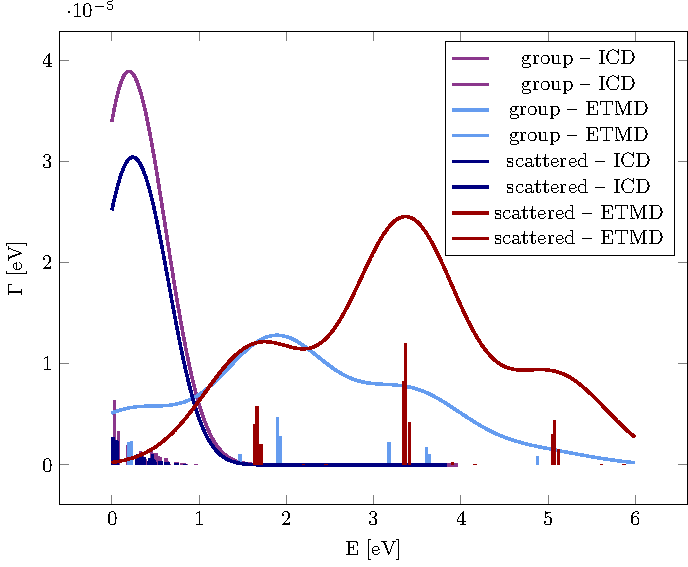
\includegraphics[width=8.5cm]{pics/ar_3_6in.pdf}
 \caption{Simulated ICD and ETMD electron spectra for clusters consisting of
          55 atoms out of which 6 are xenon atoms. These are either clustered
          (group) on one side of the cluster of evenly distributed
          inside the cluster (scattered). In both cases the ETMD peaks are
          clearly visible in the spectra.}
 \label{figure:ar_3_6in}
\end{figure}


\begin{figure}[h]
 \centering
 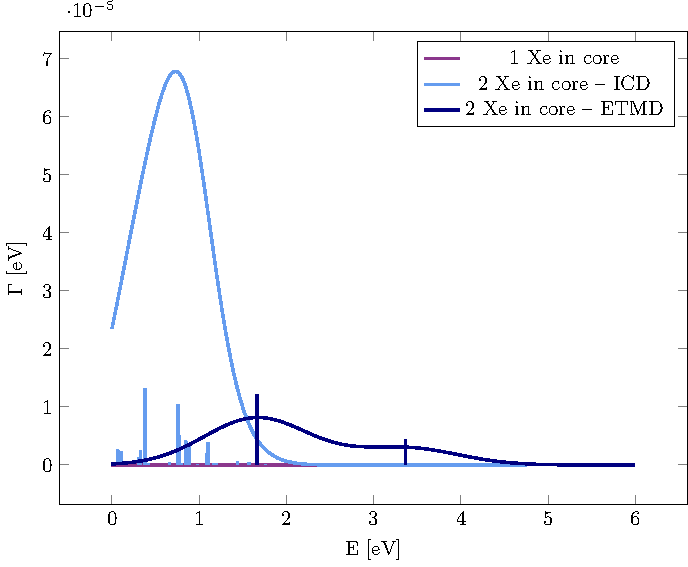
\includegraphics[width=8.5cm]{pics/xe_3_in.pdf}
 \caption{Simulated ICD and ETMD electron spectra for argon clusters with
          one or two atoms in the core of the cluster. In case of the xenon
          atom inhabiting the central position of the cluster for a 13 atoms
          cluster (not shown here) and a 55 atoms cluster all channels are closed
          for all pairs, which leads to no signal. For those clusters with two
          xenon atoms in the core the first ICD channel is open for some pairs
          and additionally ETMD is possible for multiple triples. Due to a
          different distance distribution compared to the clusters with an argon
          core the ICD peak is shifted to higher kinetic energies.}
 \label{figure:xe_3_in}
\end{figure}

\begin{figure}[h]
 \centering
 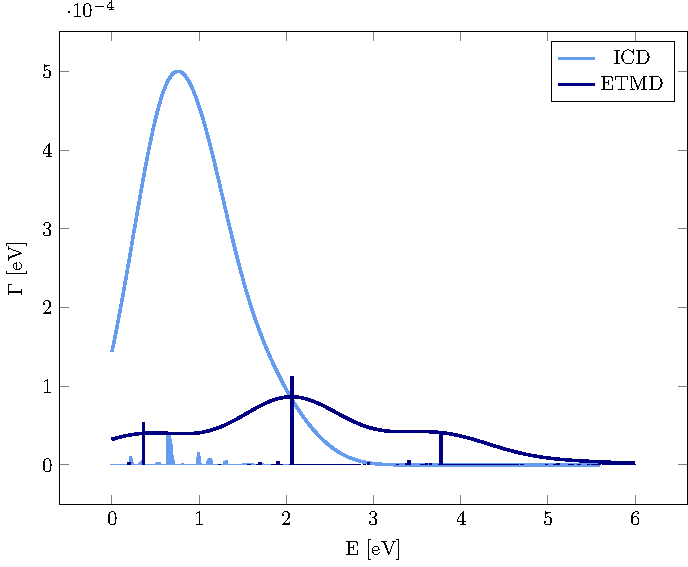
\includegraphics[width=8.5cm]{pics/xe_8_1lay.pdf}
 \caption{Simulated ICD and ETMD electron spectra for a large cluster consisting
          of a xenon core of 1415 atoms surrounded by two complete layers of
          argon atoms. The ICD and ETMD peak overlap such, that the peak structure
          might not be visible.}
 \label{figure:xe_8_lay1}
\end{figure}
